\section[Reguläre Sprachen und endliche Automaten]{Reguläre Sprachen und endliche Automaten\datenote{21.10.16}}
Endliche Automaten sind ein einfaches, formales Maschinenmodell.
Ein endlicher Automat $A$ berechnet, für eine bestimmte Sprache $L(A)$, ob ein gegebenes Wort $w$ in ihr enthalten ist (Wortproblem, $w \in L(A)$ ?).
Die Berechnungen, die sich mit endliche Automaten ausdrücken lassen sind stark beschränkt, allerdings erlaubt diese Einschränkung \emph{die Entscheidung} von Fragen wie dem Wortploblem oder dem Leerheitsproblem ($L(A)\neq\varnothing$).
D.h.\ f"ur jede dieser Fragen existiert ein Algorithmus.

\subsection{Endliche Automaten}
Wir beschreiben zunächst die Bestandteile eines endlichen Automaten:


\begin{description}
\item[Endliches Band] 
(read-only, jede Zelle enth"alt ein $a_i\in\Sigma$, der Inhalt des Bandes ist das \emph{Eingabewort}, bzw.\ die \emph{Eingabe})

\begin{figure}[H]\centering
	\begin{tikzpicture}
		\node (A) [block]{$a_0$};
		\node (B) [block,right=of A] {$\dots$};
		\node (C) [block,right=of B] {$a_n$};

    \node (L) [above=of A, node distance = 0.25cm] {Lesekopf};
    \draw[->] (L) -- (A);
	\end{tikzpicture}
	\caption{Endliches Band}
\end{figure}
\vspace{-1em}
\item[Lesekopf] ~\\
  \vspace{-\baselineskip}
  \begin{itemize}
	\item Der \emph{Lesekopf} zeigt auf ein Feld des Bandes, oder hinter das letzte Feld.
	\item Er bewegt sich feldweise nach rechts; andere Bewegungen (vor- bzw.\ zurückspulen) sind nicht möglich.
	\item Wenn er hinter das letzte Zeichen zeigt, \emph{stoppt} der Automat.
    Er muss sich nun ,,entscheiden'' ob er das Wort \emph{akzeptiert} oder nicht.
  \end{itemize}
\item[Zustände] $q$ aus \emph{endlicher} Zustandsmenge $Q$.
\item[Startzustand] $q_0 \in Q$.
\item[Akzeptierende Zustände] $F \subseteq Q$ 
\item[Transitionsfunktion] Im Zustand $q$ beim Lesen von $a$ gehe nach Zustand $\delta(q) = q'$.
\end{description}
Der endliche Automat akzeptiert eine Eingabe, falls er in einem akzeptierenden Zustand stoppt.

% Spiral - By Keven Law - originally posted to Flickr as What's your Colour???, CC BY-SA 2.0, https://commons.wikimedia.org/w/index.php?curid=6851868
% Bunch - By Mariajudit - Own work, CC BY-SA 4.0, https://commons.wikimedia.org/w/index.php?curid=48726001
% Almond - By Michelle Naherny - Own work, CC BY-SA 4.0, https://commons.wikimedia.org/w/index.php?curid=44361114
\needspace{5\baselineskip}
\begin{Bsp}Aufgabe: 
  \\
  \label{Bsp:3.1}
  ,,Erkenne alle Stapel von Maccarons in denen höchstens ein grüner Maccaron vorkommt.''
\begin{center}
  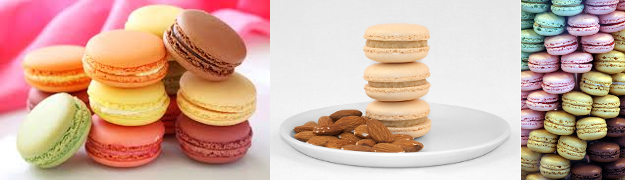
\includegraphics[scale=0.4]{macaron-stacks.png}~\footnote{
  \tiny Von links nach rechts: \\
By Mariajudit - Own work, CC BY-SA 4.0, https://commons.wikimedia.org/w/index.php?curid=48726001
  \\
By Michelle Naherny - Own work, CC BY-SA 4.0, https://commons.wikimedia.org/w/index.php?curid=44361114
  \\
By Keven Law - originally posted to Flickr as What's your Colour???, CC BY-SA 2.0, https://commons.wikimedia.org/w/index.php?curid=6851868
}
% Bunch - By Mariajudit - Own work, CC BY-SA 4.0, https://commons.wikimedia.org/w/index.php?curid=48726001
% Almond - By Michelle Naherny - Own work, CC BY-SA 4.0, https://commons.wikimedia.org/w/index.php?curid=44361114

\end{center}
Ein passendes Alphabet wäre $\Sigma = \{\mathtt{grün} , \mathtt{nicht-grün} \}$.
Wir definieren die folgenden Zustände.
(die Metapher hier ist: ,,wenn ich mehr als einen grünen Maccaron esse wird mir übel, und das wäre nicht akzeptabel'')
\begin{center}
\begin{tabular}{cl}
  Zustand & Bedeutung \\
  \hline
  $q_0$& ,,alles gut'' \\
  $q_1$& ,,mir wird schon flau'' \\
  $q_2$& ,,mir ist übel''
\end{tabular}
\end{center}
Der Startzustand ist $q_0$.
Akzeptierende Zustände sind $q_0$ und $q_1$.
Die Transistionsfunktion $\delta$ ist
\begin{center}
\begin{tabular}{cccl}
  &\texttt{grün} & \texttt{nicht-grün} \\
  \hline
  $q_0$ & $q_1$ & $q_0$ & wechsle nach $q_1$ falls \texttt{grün}, ansonsten verweile \\
  $q_1$ & $q_2$ & $q_1$ & wechsle nach $q_2$ falls \texttt{grün}, ansonsten verweile \\
  $q_2$  & $q_2$ & $q_2$ & verweile, da es nichts mehr zu retten gibt
\end{tabular}
\end{center}
\end{Bsp}

% \begin{Bsp}
% 	$L=\{w\in\{0,1\}^* \mid w \text{ enthält gerade Anzahl von 0 und gerade Anzahl von 1}\}$

% 	\begin{minipage}[t]{.4\textwidth}\centering\vspace{0pt}
% 	    \captionsetup{type=figure}
% 		\begin{tikzpicture}[circle/.style={
% 			shape=circle,
% 			minimum size=0.5cm,
% 			text=black, draw,
% 			text width=0.5cm,
% 			align=center}]
% 			\node (v1) at (-3.5,3.5) {};
% 			\node [circle,double] (v2) at (-2.5,3) {$q_{00}$};
% 			\node [circle] (v3) at (0.5,3) {$q_{01}$};
% 			\node [circle] (v4) at (0.5,0.5) {$q_{10}$};
% 			\node [circle] (v5) at (-2.5,0.5) {$q_{11}$};
% 			\draw [->] (v1) edge (v2);
% 			\draw [->] (v2) edge [bend left=15] node[auto] {1} (v3);
% 			\draw [->] (v3) edge [bend left=15] node[auto] {1} (v2);
% 			\draw [->] (v3) edge [bend left=15] node[auto] {0} (v4);
% 			\draw [->] (v4) edge [bend left=15] node[auto] {0} (v3);
% 			\draw [->] (v2) edge [bend left=15] node[auto] {0} (v5);
% 			\draw [->] (v5) edge [bend left=15] node[auto] {0} (v2);
% 			\draw [->] (v5) edge [bend left=15] node[auto] {1} (v4);
% 			\draw [->] (v4) edge [bend left=15] node[auto] {1} (v5);
% 		\end{tikzpicture}
% 		\captionof{figure}{Automat zu $L$}
% 	\end{minipage}\begin{minipage}[t]{.55\textwidth}\vspace{0pt}
% 	Graphische Darstellung $\hat=$ gerichteter Graph mit Knoten $Q$ und markierten Kanten gemäß $\delta$.\\
% 	$Q=\{q_{00},q_{01},q_{10},q_{11}\}$\\
% 	$q_{00}$ einziger akzeptierender Zustand ($F=\{q_{00}\}$)
% 	\end{minipage}
	
% 	\begin{tabular}{M{l}|M{l}|M{l}l @{\quad}l}
% 		& 0 & 1 &\\ \cline{1-3}
% 		q_{00} & q_{10} & q_{01} && gerade Anzahl von 0 und 1 gesehen\\
% 		q_{01} & q_{11} & q_{00} && gerade \ruleplaceholder{\widthof{Anzahl von 0}}, ungerade Anzahl von 1 gesehen\\
% 		q_{10} & q_{00} & q_{11} && ungerade \ruleplaceholder{\widthof{Anzahl von 0}}, gerade \ruleplaceholder{\widthof{Anzahl von 1 gesehen}} \\
% 		q_{11} & q_{01} & q_{10} && ungerade \ruleplaceholder{\widthof{Anzahl von 0}}, ungerade \ruleplaceholder{\widthof{Anzahl von 1 gesehen}}
% 	\end{tabular}
% \end{Bsp}
\begin{Def}[\acs*{DEA}]
	Ein \emph{\acf{DEA}}, (\acsu{DFA} $\hat=$ \acl{DFA}) ist ein 5-Tupel
	\[ M= (Q,\Sigma,\delta,q_0,F) \]
	\begin{itemize}
		\item $Q$ \emph{endliche} Zustandsmenge
		\item $\Sigma$ \emph{endl.} Alphabet
		\item $\delta:Q\x\Sigma\->Q$ Transitionsfunktion
		\item $q_0\in Q$ Startzustand
		\item $F\subseteq Q$ akzeptierende Zustande
	\end{itemize}
\end{Def}

DEAs lassen sich auch graphisch darstellen.
Dabei gibt man für den Automaten einen gerichteten Graphen an.
Die Knoten Graphen sind die Zustände und mit Zeichen gelabelte Kanten zeigen welchen Zustandsübergang die Transitionsfunktion für das nächste Zeichen erlaubt.
Der Startzustand ist mit einem ungelabelten Pfeil markiert und finale Zustände sind doppelt eingekreist.
Hier ist die graphische Darstellung von $A_{\mathtt{Maccaron}}$ aus Beispiel \ref{Bsp:3.1}

\begin{center}
\begin{tikzpicture}[node distance = 3cm]
  \node[state, accepting] (0) {$q_0$};
  \node[state, accepting, right of = 0] (1) {$q_1$};
  \node[state, right of = 1] (2) {$q_2$};

  \node[left of = 0, node distance = 1cm] (start){}; 
  \draw[->] (start) to (0);

  \draw[->] (0) to node[above] {\texttt{grün}} (1);
  \draw[->, loop above] (0) to node[above] {\texttt{nicht-grün}} (0);

  \draw[->] (1) to node[above] {\texttt{grün}} (2);
  \draw[->, loop above] (1) to node[above] {\texttt{nicht-grün}} (1);

  \draw[->, loop right] (2) to node[right]{\texttt{grün}, \texttt{nicht-grün}} (2);
\end{tikzpicture}
\end{center}

DEAs charakterisieren die Sprachen durch die Menge an Wörtern, die sie akzeptieren.
\begin{Bsp}
    Sei $M=(Q,\Sigma,\delta,q_0,F)$ ein DEA.
    \begin{itemize}
    \item Wenn $F=Q$, dann ist $L(M)=\Sigma^*$.
    \item Wenn $F=\emptyset$, dann ist $L(M)=\emptyset$.
    \end{itemize}
\end{Bsp}
\begin{Def}[name={[Erweiterung von $\delta$ auf Worte]}]
	Die Erweiterung von $\delta:Q\x\Sigma\->Q$ auf Worte $\hat{\delta}: Q\x\Sigma^*\->Q$ ist induktiv definiert durch
  \begin{enumerate}
  \item $\hat\delta(q,\Eps) =q$ (Wortende erreicht)
  \item $\hat\delta(q,aw)=\hat\delta(\delta(q,a),w)$ (Rest im Folgezustand verarbeiten)
  \end{enumerate}
\end{Def}
\begin{Def}[name={[Die durch einen \acs*{DEA} erkannte Sprache]}]
	Sei $M=(Q,\Sigma,\delta,q_0,F)$\\
	Die \emph{von $M$ erkannte Sprache} ist
	\[ L(M) = \{ w\in\Sigma^* \mid \hat\delta(q_0,w)\in F \} \]
	Eine durch einen \ac{DEA} erkannte Sprache heißt \emph{regulär}.
\end{Def}
Es folgen zwei Beispiele für reguläre Sprachen:
\begin{Bsp} 
\label{bsp:3.1}
	$L=\{w\in\{0,1\}^* \mid w \text{ enthält gerade Anzahl von 0 und gerade Anzahl von 1}\}$
  \begin{center}
		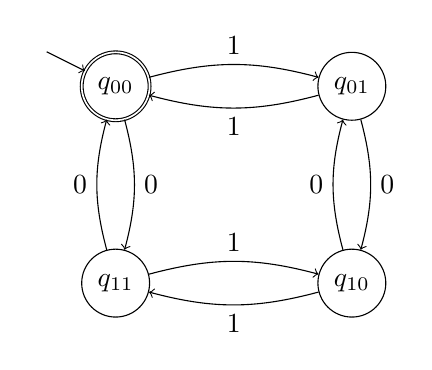
\begin{tikzpicture}[circle/.style={
			shape=circle,
			minimum size=0.5cm,
			text=black, draw,
			text width=0.5cm,
			align=center}]
			\node (v1) at (-3.5,3.5) {};
			\node [circle,double] (v2) at (-2.5,3) {$q_{00}$};
			\node [circle] (v3) at (0.5,3) {$q_{01}$};
			\node [circle] (v4) at (0.5,0.5) {$q_{10}$};
			\node [circle] (v5) at (-2.5,0.5) {$q_{11}$};
			\draw [->] (v1) edge (v2);
			\draw [->] (v2) edge [bend left=15] node[auto] {1} (v3);
			\draw [->] (v3) edge [bend left=15] node[auto] {1} (v2);
			\draw [->] (v3) edge [bend left=15] node[auto] {0} (v4);
			\draw [->] (v4) edge [bend left=15] node[auto] {0} (v3);
			\draw [->] (v2) edge [bend left=15] node[auto] {0} (v5);
			\draw [->] (v5) edge [bend left=15] node[auto] {0} (v2);
			\draw [->] (v5) edge [bend left=15] node[auto] {1} (v4);
			\draw [->] (v4) edge [bend left=15] node[auto] {1} (v5);
		\end{tikzpicture}
  \end{center}
\end{Bsp}
\begin{Bsp}\label{bsp:3.2}
	
	Sei $A\ge 0$ nat. Zahl, $\Sigma=\{0,1,\dots,A\}$
	\begin{equation*}
		L = \{ a_1\dots a_n \mid \exists J\subseteq \{1,\dots,n \},\ \sum_{i\in J} a_i = A \} \subseteq \Sigma^* 
	\end{equation*}
	D.h. gegeben eine Liste von Zahlen $\in\Sigma$.
	Akzeptiere diejenigen Listen, für die eine Teilliste existiert, deren Summe genau $A$ ist.
	\begin{align*}
		Q &=\Powerset\{0,1,\dots,A\} \\
		\delta(q,a) &= q \cup \{ x\in \{0,\dots,A\} \mid x-a \in q \} \\
		q_0 &=\{0\} \\
		F &= \{ q\in Q \mid A \in q \}
	\end{align*}
  $q \in Q$ bezeichnet die Menge an möglichen Summen $\le A$, die mit den bisher gelesenen Zeichen gebildet werden kann.
  Die Transitionsfunktion $\delta$ fügt die Summen zum aktuellen Zustand hinzu, die sich durch addieren der aktuell gelesenen Ziffer zu den alten Möglichkeiten ergeben.
\end{Bsp}
\begin{Bsp}\label{bsp:3.3}
	Beispiel f"ur eine nicht-regul"are Sprache.
	\begin{equation*}
		L = \{ 0^n1^n \mid n\in\N \} 
	\end{equation*}
	erkennbar durch \ac{TM} die immer anhält, \emph{aber nicht} von einem \ac{DEA} [\emph{nicht} regulär] akzeptiert werden kann.
	\begin{proof}
		Angenommen $L=L(M)$ für \ac{DEA} $M=(Q,\Sigma,q_0,\delta,F)$
		
		Beobachtung: $\exists m\neq n$, sodass $\hat\delta(q_0,0^m)=\hat\delta(q_0,0^n)=q'$ weil $Q$ endlich.
		\begin{itemize}
			\item Falls nun $\hat\delta(q',1^m)\in F$, dann ist auch $\hat\delta(q_0,0^n1^m)\in F$ und somit $0^n1^m\in L(M)$ mit $n\neq m\ \lightning$
			\item Falls $\hat\delta(q',1^m)\notin F$, dann gilt auch $\hat\delta(q_0,0^m1^m)\notin F$ und somit $0^m1^m \notin L$ $\lightning$
		\end{itemize}
		Also kann $M$ nicht existieren!
	\end{proof}
\end{Bsp}

\subsection{Minimierung endlicher Automaten}
 \datenote{26.10.16}

Betrachte den Automaten aus Beispiel \ref{bsp:3.2}.
Sei $A =4$, $\Sigma = \{0, 1, 2, 3, 4\}$ mit Zustandsmenge $Q = \Powerset(\Sigma)$.
D.h.\ unter anderem: $\{0, 1, 3\} \in Q$.
Hier ist ein Ausschnitt aus dem Zustandsdiagramm:

\begin{center}
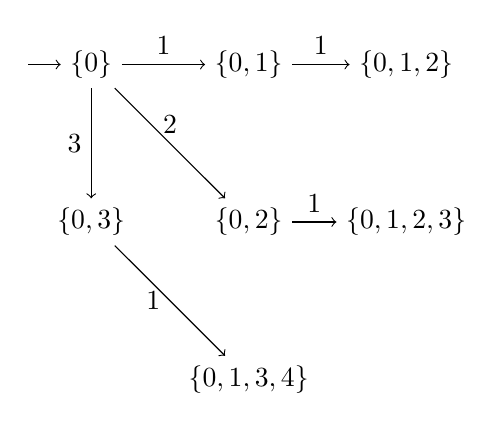
\begin{tikzpicture}[node distance = 2cm]
  \node (0) at (0, 0) {$\{0\}$};
  \node[below of = 0] (03) {$\{0,3\}$};
  \node[right of = 03] (02) {$\{0,2\}$};
  \node[below of = 02] (0134) {$\{0,1,3,4\}$};
  \node[right of = 0] (01) {$\{0,1\}$};
  \node[right of = 01] (012) {$\{0,1,2\}$};
  \node[below of = 012] (0123) {$\{0,1,2, 3\}$};

   \draw[->] (- 0.8, 0) to (0);
  \draw[->] (0) to node[left] {$3$} (03);
  \draw[->] (0) to node[above] {$2$} (02);
  \draw[->] (0) to node[above] {$1$} (01);
  \draw[->] (03) to node[left] {$1$} (0134);
  \draw[->] (01) to node[above] {$1$} (012);
  \draw[->] (02) to node[above] {$1$} (0123);
\end{tikzpicture}
\end{center}
Es ist zu bemerken, dass manche Zustände von $Q$ nie erreicht werden können, z.B.\ $\emptyset$.
Sei für die folgenden Überlegungen $M = (Q, \Sigma, \delta, q_0, F)$ ein DEA.

\begin{Def}
  Ein Zustand $q \in Q$ ist \emph{erreichbar}, falls ein $w \in \Sigma^*$ existiert, so dass $\hat \delta(q_0, w) = q$.
  $M$ heißt \emph{reduziert}, falls alle Zustände erreichbar sind.
\end{Def}
\begin{Satz}
  Die Menge der erreichbaren Zustände kann in $O(|Q|*|\Sigma|)$ berechnet werden.
\end{Satz}
\begin{proof}~\\
  \vspace{-\baselineskip}
  \begin{itemize}
  \item Fasse $A$ als Graphen auf.
  \item Wende Tiefensuche an, markiere dabei alle besuchten Zustände.
  \item Die markierten Zustände ist die Menge der erreichbaren Zustände.
  \end{itemize}
\end{proof}

\ldots 



\draftnote{28.10.16}

\emph{Beobachtung:} Auch ein Automat mit lauter erreichbaren Zuständen muss nicht minimal sein

\begin{Bsp}\label{Bsp:3.4}\
	\begin{figure}[H]\centering
		\begin{tikzpicture}
			\node (start) at (-4,1.5) {};
			\node (q0) [circle,double] at (-3,1) {$q_0$};
			\node (q1) [circle,double] at (-0.5,1) {$q_1$};
			\node (q2) [circle] at (2,1) {$q_2$};
			\node (q3) [circle] at (3.5,1) {$q_3$};
			\draw [->] (start) edge (q0);
			\draw [->] (q0) edge[loop above] node {0} (q0);
			\draw [->] (q0) edge node [auto] {1} (q1);
			\draw [->] (q1) edge[loop above] node {0} (q1);
			\draw [->] (q1) edge node [auto] {1} (q2);
			\draw [->] (q2) edge[loop above] node {1} (q2);
			\draw [->] (q2) edge[bend left] node [auto] {0} (q3);
			\draw [->] (q3) edge[bend left] node [auto] {1,0} (q2);
		\end{tikzpicture}\\
		höchstens eine "`1"'
		\caption{Automat zu Bsp. \ref{Bsp:3.4}}
	\end{figure}
	Erkennt die gleiche Sprache wie in \eqref{bsp:3.1}, hat nur erreichbare Zustände, aber mehr Zustände als in \eqref{bsp:3.1}.
	
	\emph{Beobachtung:} $q_2$ und $q_3$ verhalten sich gleich in dem Sinn, dass
	\[ \forall w: \hat\delta(q_2,w) \notin F\text{ und }\hat\delta(q_3,w)\notin F \]
\end{Bsp}
%
%\stepcounter{Def}
%
\begin{Def}[name={[Äquivalenz von \acs*{DFA}-Zuständen]}] %\rlnote{Def.-Num. überprüfen}
	Zwei Zustände $q,p\in Q$ eines \ac{DFA} sind \emph{äquivalent}, geschrieben $p\equiv q$, falls $\forall w\in\Sigma^*$, $\hat\delta(p,w)\in F \<=> \hat\delta(q,w)\in F$
\end{Def}
%\stepcounter{lemma}

\begin{lemma}[name={[$\equiv$ ist Äquivalenzrelation]}] %\rlnote{Satz = Lemma-Nummer: 3.2 statt 3.1?}
	$\equiv$ ist Äquivalenzrelation\\
	\framebox{\parbox{.96\linewidth}{Eine Relation ist genau dann eine Äquivalenzrelation, wenn sie reflexiv, transitiv und symmetrisch
	ist.}}
\end{lemma}
\begin{proof} $\equiv$ ist offensichtlich reflexiv.
	
	$\begin{rcases}
	\text{transitiv}\\
	\text{symmetrisch}
	\end{rcases}$ wegen \<=>
	
	Also $q_2,q_3$ aus \autoref{Bsp:3.4} sind äquivalent.
\end{proof}
\begin{Erinnerung}
Hauptlemma "uber "Aquivalenzrelationen
\begin{align*}
	[q] &= \{p\in Q \mid p \equiv q\} &&[q] \text{ ist Äquivalenzklasse von }q
\end{align*}
"Aquivalenzklassen sind paarweise disjunkt:

F"ur alle $ p,q\in Q$ gilt entweder $[p]=[q]$ oder $[p]\cap[q] = \emptyset$ (folgt aus Transitivität).

D.h. $Q$ wird in disjunkte Äquivalenzklassen aufgeteilt. Anzahl der Äquivalenzklassen ist der \textbf{Index}.
\end{Erinnerung}

\eqref{bsp:3.1}:
\begin{minipage}{.5\textwidth}
    \captionsetup{type=figure}
	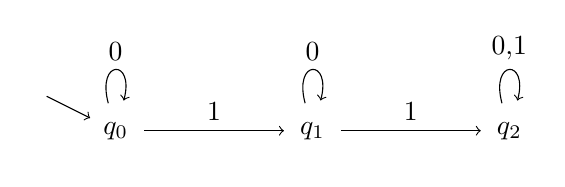
\begin{tikzpicture}
		\node (start) at (-4,1.5) {};
		\node (q0) [circle,double] at (-3,1) {$q_0$};
		\node (q1) [circle,double] at (-0.5,1) {$q_1$};
		\node (q2) [circle] at (2,1) {$q_2$};
		\draw [->] (start) edge (q0);
		\draw [->] (q0) edge[loop above] node {0} (q0);
		\draw [->] (q1) edge[loop above] node {0} (q1);
		\draw [->] (q2) edge[loop above] node {0,1} (q2);
		\draw [->] (q0) edge node [auto] {1} (q1);
		\draw [->] (q1) edge node [auto] {1} (q2);
	\end{tikzpicture}
	\captionof{figure}{Automat zu \eqref{bsp:3.1}}
\end{minipage}

Allgemein gilt f"ur alle $p,q\in Q$:
\begin{align}
\label{eqn:delta-wohldefiniert}
	p &\equiv q \=> \forall a\in\Sigma:\ \delta(p,a)\equiv\delta(q,a)
\end{align}
Denn
\begin{align*}
	p \equiv q  
	& \<=> \forall w\in\Sigma^*: \hat\delta(p,w)\in F \<=> \hat\delta(q,w) \in F\\
	& \<=> (p\in F \<=> q \in F) \land \forall a\in \Sigma: \forall w\in\Sigma^*:
	\hat\delta(p,aw)\in F \<=> \hat\delta(q,aw)\in F\\
	&\=>  \forall a\in\Sigma: \forall w\in\Sigma^*: \hat\delta(\delta(p,a),w)\in F \<=> \hat\delta(\delta(q,a),w)\in F\\
	& \<=>\forall a\in\Sigma: \delta(p,a)\equiv\delta(q,a)
\end{align*}
Also können wir äquivalente Zustände zusammenfassen und Transitionen verschmelzen, wie in der folgenden Definition formalisiert.
\begin{Def}[name={[Äquivalenzklassenautomat]}]
	Der Äquivalenzklassenautomat $M'=(Q',\Sigma,\delta',q_0',F')$ zu $M$ ist bestimmt durch:
	\begin{align*}
		Q' &= \{[q]\mid q\in Q\} & \delta'([q],a) &= [\delta(q,a)]\\
		q_0' &= [q_0] & F'&=\{[q]\mid q\in F \}
	\end{align*}
\end{Def}
Dabei ist $[q]=\{p\in Q \mid p\equiv q\}$
\begin{Satz}[name={[Äquivalenzklassenautomat ist wohldefiniert]}]
	Der Äquivalenzklassenautomat ist wohldefiniert und $L(M)=L(M')$.
\end{Satz}
\begin{proof}\ 
	\begin{enumerate}
		\item Wohldefiniert: zu zeigen $\delta'([q],a) =[\delta(q,a)]$ ist nicht abhängig von der Wahl des Repräsentanten $q\in [q]$. Das folgt direkt aus \eqref{eqn:delta-wohldefiniert} gezeigt.
		\item $L(M)=L(M')$ zeige für alle $w\in\Sigma^*$ und alle $q$: $\hat\delta(q,w)\in F \<=> \hat\delta'([q],w)\in F'$\\
		Induktion über $w$:\\
		I.A. $w=\Eps$: $\hat\delta(q,\Eps)=q\in F \<=> \hat\delta'([q],\Eps)=[q]\in F'$ nach Definition.\\
		I.V.: $\forall w'\in\Sigma$, $\forall q\in Q$, $\hat\delta(q,w')\in F \<=> \hat\delta'([q],w')\in F'$\\
		I.S.: \begin{align*}
		\hat\delta(q,aw')\in F &\<==> \hat\delta(\delta(q,a),w')\in F\\ &\xLeftrightarrow{I.V.} \hat\delta'([\delta(q,a)],w')\in F'\\
		&\<==> \hat\delta'(\delta'([q],a),w')\in F'\\
		&\<==> \hat\delta'([q],a w')\in F'
		\end{align*}
		Also f"ur $q=q_0$: $\forall w\in\Sigma^*$, $w\in L(M)\<==> \hat\delta(q_0,w) \in F \<=> \hat\delta'([q_0],w) \in F' \<==> w\in L(M')$
	\end{enumerate}
\end{proof}
\emph{Bem:} Die Konstruktion von $M'$ kann in $O(|Q||\Sigma|\log|Q|)$ passieren.

Warum ist nun der Äquivalenzklassenautomat minimal?\\
\-> Satz von Myhill-Nerode
\begin{Def}[name={[Rechtsinvariante Äquivalenzrelation]}]
	Eine Äquivalenzrelation $R\subseteq\Sigma^*\x\Sigma^*$ heißt rechtsinvariant, falls
	\[ (u,v)\in R \=> \forall w\in\Sigma^*,(u\cdot w,v\cdot w) \in R \]
\end{Def}
%\setcounter{Bsp}{5}
\begin{Bsp} %\rlnote{Bsp.-Num. überprüfen (3.6)}
	Für einen \ac{DEA} $M$ definiere
	\[ R_M = \{(u,v) \mid \hat\delta(q_0,u)=\hat\delta(q_0,v)\} \]
	\begin{itemize}
		\item ist Äquivalenzrelation
		\item ist rechtsinvariant
		\item Anzahl der Äquivalenzklassen(Index von $R_M$)\\
		= Anzahl der "`nützlichen"' Zustände, die von $q_0$ erreichbar sind.
	\end{itemize}
\end{Bsp}
\begin{Bsp}
	Für eine Sprache $L\subseteq \Sigma^*$ definiere die Nerode Relation
	\[ R_L = \{(u,v) \mid \forall w\in\Sigma^*: uw\in L \<=> vw\in L \} \]
	\begin{itemize}
		\item ist Äquivalenzrel.
		\item ist rechtsinvariant. Sei $(u,v)\in R_L$\\
		Zeige $\forall w\in\Sigma^*\ (uw,vw)\in R_L$\\
		Induktion:\\
		I.A. $w=\Eps$: $ (u\Eps,v\Eps)=(u,v)\in R_L$\\
		I.S. $w=w'a$:\\
		I.V.: $(uw', vw') \in R_L $
		\begin{align*}
			(uw',vw')\in R_L 
			&\<=> \forall z\in\Sigma^*, \quad uw'z\in L \<=> vw'z\in L\\
			&\=> \forall a\in \Sigma, z'\in\Sigma^*: uw'az'\in L \<=> vw'az'\in L\\
			& \<=>\ (uw'a,vw'a)\in R_L
		\end{align*}
	\end{itemize}
\end{Bsp}

\begin{alignat*}{2}
	&\begin{rcases}
	L=\{\Eps\} & [\Eps]\equiv[\Eps]\\
	w,v\in\Sigma^*,\ w,v\ne\Eps & [w]=[v]
	\end{rcases} &\ &\text{Index}= 2\\
	&L = \varnothing, L= \Sigma^* &&\text{Index}= 1
\end{alignat*}

\begin{Satz}[Nerode] % 3.4
	Die folgende Aussagen sind äquivalent:
	\begin{enumerate}
		\item\label{itm:Nerode1} $L\subseteq \Sigma^*$ wird von \ac{DEA} akzeptiert.
		\item\label{itm:Nerode2} $L$ ist Vereinigung von Äquivalenzklassen einer rechtsinvarianten Äquivalenzrel. mit \emph{endlichem} Index.
		\item\label{itm:Nerode3} Die Nerode Relation $R_L$ hat \emph{endlichen} Index
	\end{enumerate}
\end{Satz}

\begin{proof}
	(1) \=> (2): Sei $M$ ein \ac{DEA} mit $L(M)=\{w \mid \hat\delta(q_0,w)\in F \} = \bigcup\limits_{q\in F}[q]_M$
	wenn $[q]_M =\{ w \mid \hat\delta(q_0,w)=q \}$\\
	Äquivalenzklassen und \#Klassen$\leq|Q|$ endl.
	
	(2) \=> (3): Sei $R$ rechtsinv. Äquivrel. mit endl. Index sodass $L=\bigcup R$-Äquivalenzklassen
	
	Sei $(u,v)\in R$. Zeige $(u,v)\in R_L $.\\
	Wegen $R$ rechtsinv. $\forall w\in\Sigma^*\ (uw,vw)\in R$
	\begin{alignat*}{2}
		&&&\forall w\in\Sigma^*: (uw,vw)\in R\\
		&\<=>&\quad&\forall w\in\Sigma^*\quad uw\text{ und $vw$ in gleicher $R$-Klasse}\\
		&\=>&&\forall w\in\Sigma^* \quad uw\in L\<=>vw\in L\\
		&\<=>&& (u,v)\in R_L\\
		&\=>&&\text{\#Klassen($R_L$)$\leq$\#Klassen($R$)}<\infty
	\end{alignat*}


    (3) \=> (1) Gegeben $R_L$\\
		Konstruiere $\A'=(Q,\Sigma,\delta',q_0',F')$
		\begin{alignat*}{3}
			&&Q' &= \{ [w]_{R_L} \mid w\in \Sigma^* \} &\quad& \text{endlich, weil index($R_L$) endl.}\\
			&&\delta'([w],a) &= [wa] && \text{wohldefiniert, da $R_L$ rechtsinvariant}\\
			&&q_0' &= [\Eps]\\
			&&F' &= \{ [w] \mid w\in L \}\\
			\shortintertext{Zeige $L(\A')=L$, d.h. }
			&\forall w\in \Sigma^* &: w\in L(\A') &\<=> \hat\delta([\Eps],w)\in F'\\
			&&&\overset{???}{\<=>} [w]\in F' \\
			&&&\<=> w\in L
		\end{alignat*}
		Zeige nun noch, dass $???$ gilt: $\hat\delta([\Eps], w) = [w]$. 
		Daf"ur m"ussen wir wie folgt verallgemeinern um eine funktionierende Induktionsvoraussetzung zu erhalten.
		\begin{alignat*}{3}
			&&\forall w\in\Sigma^* &:
			\forall v\in\Sigma^* : \hat\delta'([v],w) = [v\cdot w]\\
			\shortintertext{Induktion über $w$}
			&\text{I.A.: }& \Eps &: \hat\delta'([v],\Eps) = [v]=[v\cdot\Eps]\\
			&\text{I.S.: }& \hat\delta'([v],aw') &= \hat\delta'(\delta'([v],a),w')\\
			&&&= \hat\delta'([v\cdot a],w')\\
			&&&\overset{\mathrlap{\text{I.V.}}}{=} [va\cdot w']\\
			&&&= [v\cdot \underbrace{aw'}_{=w}]
		\end{alignat*}
		Das gewünschte Ergebnis \framebox{???} ergibt sich für $v=\Eps$. \qedhere
\end{proof}
%
\setcounter{Korollar}{4}
\begin{Korollar}
	Der im Beweisschritt (3) \=> (1) konstruierte Automat $\A'$ ist minimaler Automat für $L$.
\end{Korollar}
\begin{proof}
	$L$ regulär. Sei $\A$ \emph{beliebiger \ac{DFA} mit $L=L(\A)$}\\
	$\begin{rcases}
	\A\text{ induziert }R_\A\text{ mit}\\
	|Q|\geq\text{index}(R_\A)
	\end{rcases}$ $\ref{itm:Nerode1} \overset{vgl.}{\<=>} \ref{itm:Nerode2}$
	
	In \ref{itm:Nerode2} \=> \ref{itm:Nerode3}: $R_\A\subseteq R_L$,\ index($R_\A$) $\geq$ index($R_L$)\\
	In \ref{itm:Nerode3} \=> \ref{itm:Nerode1} $A'$ mit $|Q'|=\text{index}(R_L) \leq \text{index}(R_\A)\leq |Q|$
	
	Minimalität von $A'$ folgt aus freier Wahl von $\A$
\end{proof}

Angenommen $\exists\,\A$ mit $L=L(\A)$ und $|\A|<|\A'|$\\
Nach Folgerung gilt aber
\[ |\A'| \leq |\A|\ \lightning \]

\subsection{\acf{PL} für reguläre Sprachen} %\rlnote{subsection \# (3.3)?}
\datenote{26.10.16 (Eingeschoben)}
Suche: Notwendiges Kriterium für Regularität
\begin{Bsp*}
		$L = \{ w\in \{0,1\}^* \mid \operatorname{bin}(w)\equiv_3 0\}$ ist regulär, dabei ist "`bin"' die Dekodierung von einem Bitstring in eine nat"urliche Zahl.
    \begin{center}
		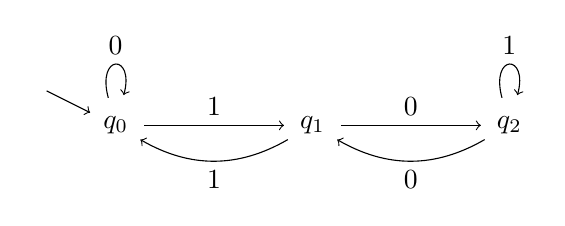
\begin{tikzpicture}
			\node (start) at (-4,1.5) {};
			\node (q0) [circle, double] at (-3,1) {$q_0$};
			\node (q1) [circle] at (-0.5,1) {$q_1$};
			\node (q2) [circle] at (2,1) {$q_2$};
			\draw [->] (start) edge (q0);
			\draw [->] (q0) edge [loop above] node {0} (q0);
			\draw [->] (q0) edge node [auto] {1} (q1);
			\draw [->] (q1) edge [bend left] node [auto] {1} (q0);
			\draw [->] (q1) edge node [auto] {0} (q2);
			\draw [->] (q2) edge [bend left] node [auto] {0} (q1);
			\draw [->] (q2) edge [loop above] node {1} (q2);
		\end{tikzpicture}
  \end{center}
  \begin{itemize}
  \item Es gilt offensichtlich, dass $11 \in L$
  \item Es auch, dass $1 \underline{0 0} 1 \in L$.
  \item Der Automat hat eine Schleife bei $\hat\delta({q_1,00}) = q_1$, die mehrfach ,,abgelaufen'' werden kann ohne die Akzeptanz zu beinflussen.
  \item Also gilt auch $100001 \in L$,
  \item und im Allgemeinen $\forall i\in\N: 1(00)^i1 \in L$
  \end{itemize}
\end{Bsp*}

\begin{lemma}[Pumping Lemma]\label{lem:pumping}
	Sei $L$ regulär:
	\begin{alignat*}{2}
		&\exists n\in\N,\ n>0\quad \forall z\in L,\ |z|\geq n:\\
		&\exists u,v,w\in\Sigma^* :\\
		&z = uvw,\ |uv| \leq n,\ |v| \geq 1\\
		\text{sodass }& \forall i\in\N:\ uv^iw\in L
	\end{alignat*}
\end{lemma}
\vspace{-1em}
\begin{proof}
	Sei $\A=(Q,\Sigma,\delta,q_0,F)$ ein \ac{DFA} für $L$.\\
	Wähle $n=|Q|$ und $z\in L$ mit $|z|\geq n$.
	
	Beim Erkunden von $z$ durchläuft $\A\ \underbrace{|z|+1}_{\geq n+1}$ Zustände.\\
	\-> $\exists\, q$, das mehrmals besucht wird.
	
	Wähle das $q$, dessen zweiter Besuch zuerst passiert.
	\begin{alignat*}{3}
		\text{D.h.}:&\quad& \hat\delta(q_0,u)&=q &\qquad& u\text{ Präfix von }z\\
		\exists v:&& \hat\delta(q,v)&=q && uv\text{ Präfix von }z\\
		\exists w:&& \hat\delta(q,w)&\in F && uvw=z\\
		&& |v| &\geq 1\\
		&& |uv| &\leq n && \text{ergibt sich aus Wahl von }q
	\end{alignat*}
	\begin{alignat*}{2}
		\text{jetzt:}\quad &\hat\delta(q_0,uv^iw) &\quad& i\in\N\\
		&= \hat\delta(q,v^iw)\\
		&= \hat\delta(q,w) && \text{denn }\forall i: \hat\delta(q,v^i)=q\\
		&\in F \tag*{\qedhere}
	\end{alignat*}
\end{proof}
%
\begin{Bsp*}
	$L=\{0^n10^n \mid n\in\N\}$ ist nicht regulär.\\
	Sei $n$ die Konstante aus dem \ac{PL}.
	
	Wähle $z=0^n10^n$. Also $|z|=2n+1\geq n$\\
	Laut PL existieren $u$, $v$, $w$, sodass $z=uvw$ mit $|v|\geq 1, |uv|\leq n$ und $\forall i \in \N$ $uv^iw \in L$. Nach Wahl von $z$ gilt nun
  \begin{itemize}
  \item $uv = 0^m$ mit $m\leq n$
  \item $v = 0^k$ mit $k\geq 1$
  \item $w = 0^{n-m}10^n$ 
  \end{itemize}
  Betrachte $uv^2w = 0^{m+k}0^k0^{n-m}10^n = 0^{n+k}10^n \notin L$.
  Also ist $L$ nicht regulär.
  Zur Illustration:
	\begin{gather*}
		\underbrace{0\ \dots\dots\ 0}_{n} \ \underbrace{1\ \dots\dots\ 1}_{n}\\
		|\!\ruleplaceholder[u]{\widthof{0\ \dots }} \!|\! \ruleplaceholder[v]{\widthof{\dots 0}}\!|% 
		\ruleplaceholder[w]{\widthof{\ \ \ $1\ \dots\dots\ 1$}}\!|
	\end{gather*}
  
\end{Bsp*}
\begin{Bsp*}
	$L=\{0^{x^2} \mid x\in\N\}$ ist nicht regulär.\\
	Sei $n$ die Konstante aus dem \ac{PL}.
	
	Wähle $z=0^{n^2}$. Also $|z|=n^2\geq n$\\
	Laut PL existieren $u$, $v$, $w$, sodass $z=uvw$ mit $|v|\geq 1, |uv|\leq n$ und $\forall i \in \N$ $uv^iw \in L$. Nach Wahl von $z$ gilt nun
  \begin{itemize}
  \item $uv = 0^m$ mit $m\leq n$
  \item $v = 0^k$ mit $k\geq 1$
  \item $w = 0^{n^2 - m}$ mit $k\geq 1$
  \end{itemize}
  Betrachte $uv^2w = 0^{m+k}0^k0^{n^2-m} = 0^{n^2+k}$.
  Da $n^2+k$ keine Quadratzahl sein kann ist $uv^2w \not \in L$, und somit ist $L$ nicht regulär.
  Begründung: betrachte $(n+1)^2 - n^2 = n^2 + 2n + 1 - n^2 = 2n + 1$.
  Aber $k \le m \le n \le 2n + 1$.
\end{Bsp*}

\begin{Bsp*}
$L_2 = \{0^p \mid p\text{ ist Primzahl}\}$ ist nicht regulär.

Sei $n$ Konst. aus dem \ac{PL}, $p$ Primzahl mit $p \geq n$.\\
Wähle $z=0^p \in L_2$
\begin{align*}
	\ac{PL}:\ &z=uvw \text{ mit } |uv|\leq n &&,|v| \geq 1\\
	&\curvearrowright |z|= p=a+b &&, a = |uw| \quad, b= |v|\\
	&\curvearrowright |uv^iw| = a + ib &&, \text{w"ahle }i=p+1\\
	&\curvearrowright |uv^{p+1}w| = a + (p+1)b & =& a + pb + b = p+pb \text{ keine Primzahl} \\
	\text{Also } &uv^{p+1}w \notin L_2\\
	&\curvearrowright L_2\text{ nicht regulär.}
\end{align*}
\end{Bsp*}

\subsection[\acf{NEA}]{\acf{NEA}\draftnote{2.11.16}}
\begin{Bsp*} Mustererkennung\\
	kommt ein String (konsistent) in einem anderen vor?
	
	Gegeben: festes Wort $w$.\\
	Gesucht: Sprache aller Worte, in denen $w$ als Teilwort vorkommt.
	\begin{align*}
		L &= \{ v\in\Sigma^* \mid \exists u,x\in\Sigma^*, v=uwx \}\\
		\Sigma &= \{a,b,c\}\\
		& \text{konkretes Beispiel:}\\
		w &= abac
	\end{align*}
	\begin{figure}[tp]
	\centering
		\begin{tikzpicture}[>=stealth, shorten >=1pt,
				node distance=2cm, on grid, initial text=,
				every state/.style={minimum size=0pt,inner sep=0pt}
			]
			\node[state,initial] (q0) {};
			\node[state] (q1) [right of=q0] {};
			\node[state] (q2) [right of=q1] {};
			\node[state] (q3) [right of=q2] {};
			\node[state,accepting] (q4) [right of=q3] {};
			\path[->]
				(q0) edge [loop above]    node [auto]  {$b,c$}    ()
				     edge                 node [auto]  {$a$}      (q1)
				(q1) edge [loop above]    node [auto]  {$a$}      ()
				     edge [bend left]     node [auto]  {$c$}      (q0)
				     edge                 node [auto]  {$b$}      (q2)
				(q2) edge [bend left=50]  node [auto]  {$b,c$}    (q0)
				     edge                 node [auto]  {$a$}      (q3)
				(q3) edge                 node [auto]  {$c$}      (q4)
				     edge [bend right=70] node [above] {$a$}      (q1)
				     edge [bend right=40] node [above] {$b$}      (q2)
				(q4) edge [loop right]    node [auto]  {$\Sigma$} ()
			;
		\end{tikzpicture}
	\caption{DFA für $L$}
	\label{fig:dfa-teilwort}
	\end{figure}
	\hyperref[fig:dfa-teilwort]{Abbildung~\ref*{fig:dfa-teilwort}} enthält einen \ac{DFA} für die Sprache $L$. Beobachtung: nicht-trivial zu konstruieren.
	\begin{figure}[tp]\centering
		\begin{tikzpicture}[>=stealth,shorten >=1pt,
				node distance=2cm,on grid,
				initial text=
			]
			\node[state,initial] (q0) {$q_0$};
			\node[state] (q1) [right of=q0] {$q_1$};
			\node[state] (q2) [right of=q1] {$q_2$};
			\node[state] (q3) [right of=q2] {$q_3$};
			\node[state,accepting] (q4) [right of=q3] {$q_4$};
			\path[->]
				(q0) edge [loop above] node [auto] {$\Sigma$} ()
				     edge              node [auto] {$a$} (q1)
				(q1) edge              node [auto] {$b$} (q2)
				(q2) edge              node [auto] {$a$} (q3)
				(q3) edge              node [auto] {$c$} (q4)
				(q4) edge [loop above] node [auto] {$\Sigma$} ()
			;
		\end{tikzpicture}
		\caption{Bsp.: Mustererkennung}
		\label{fig:nfa-teilwort}
	\end{figure}
	
	\hyperref[fig:nfa-teilwort]{Abbildung~\ref*{fig:nfa-teilwort}} enthält einen nicht-deterministischen endlichen Automat für die Sprache $L$. Idee: Ein Wort $w$ wird akzeptiert, falls es einen mit $w$ markierten Pfad von $q_0$ zu einen akzeptierenden Zustand gibt.
	\begin{figure}[tp]
	\centering
		\begin{tikzpicture}[>=stealth,shorten >=1pt,
				node distance=2cm,on grid
			]
			\node (q0) {$\{0\}$};
			\node (q1) [right of=q0] {$\{0,1\}$};
			\node (q2) [right of=q1] {$\{0,2\}$};
			\node (q3) [right of=q2] {$\{0,1,3\}$};
			\path[->]
				(q0) edge [loop below] node [auto] {$b,c$} ()
				     edge              node [auto] {$a$} (q1)
				(q1) edge [loop below] node [auto] {$a$} ()
				(q1) edge              node [auto] {$b$} (q2)
				(q2) edge              node [auto] {$a$} (q3)
			;
		\end{tikzpicture}
	\caption{Potenzmengenkonstruktion auf dem NFA}
	\label{fig:nfa-teilwort-powerset}
	\end{figure}
	
	\hyperref[fig:nfa-teilwort-powerset]{Abbildung~\ref{fig:nfa-teilwort-powerset}} zeigt (einen Ausschnitt) aus dem deterministischen Automaten, der schematisch aus dem \acsu{NFA} in \autoref{fig:nfa-teilwort} konstruiert werden kann. Idee: bei Schritt mit Symbol $a$ ist der \ac{NFA} gleichzeitig in allen Zuständen, die durch $a$ von (der Menge der) aktuellen Zustände erreichbar sind.
	
	Variante: erkenne \textbf{Subwort} $w=a_1,\dots,a_n$
	\[ L' = \{ v\in\Sigma^* \mid \exists x_0,\dots,x_n\in\Sigma^*, v=x_0a_1x_1a_2\dots a_nx_n \} \]
	Nicht det. Automat für $L'$ mit $(w=abac)$ ist sehr einfach. Der entsprechende deterministische Automat ist deutlich komplizierter. (selbst)
	\begin{figure}[H]\centering
		\begin{tikzpicture}[>=stealth, shorten >=1pt,
				node distance=2cm, on grid, initial text=,
				every state/.style={minimum size=0pt,inner sep=0pt}
			]
			\node[state,initial] (q0) {};
			\node[state] (q1) [right of=q0] {};
			\node[state] (q2) [right of=q1] {};
			\node[state] (q3) [right of=q2] {};
			\node[state,accepting] (q4) [right of=q3] {};
			\path[->]
				(q0) edge [loop above] node [auto] {$\Sigma$} ()
				     edge              node [auto] {$a$}      (q1)
				(q1) edge [loop below] node [auto] {$\Sigma$} ()
				     edge              node [auto] {$b$}      (q2)
				(q2) edge [loop below] node [auto] {$\Sigma$} ()
				     edge              node [auto] {$a$}      (q3)
				(q3) edge [loop below] node [auto] {$\Sigma$} ()
				     edge              node [auto] {$c$}      (q4)
				(q4) edge [loop right] node [auto] {$\Sigma$} ()
			;
		\end{tikzpicture}
		\caption{Nichtdet. Automat für $L'$}
	\end{figure}
	
	Weiteres Beispiel, bei dem der deterministische Automat beweisbar exponentiell größer ist.
	\begin{align*}
		L_n &= \{ w\in\{0,1^* \mid \text{das $n$-letzte Symbol von $w$ ist 1} \}
	\end{align*}
	\begin{figure}[H]\centering
		\begin{tikzpicture}[>=stealth, shorten >=1pt,
				node distance=1.5cm, on grid, initial text=,
				every state/.style={minimum size=0pt,inner sep=0pt}
			]
			\node[state,initial] (q0) {};
			\node[state] (q1) [right of=q0] {};
			\node        (q2) [right of=q1] {\dots};
			\node[state,accepting] (q3) [right of=q2] {};
			\path[->]
				(q0) edge [loop above] node [auto] {$\Sigma$} ()
				     edge              node [auto] {1}        (q1)
				(q1) edge              node [auto] {$\Sigma$} (q2)
				(q2) edge              node [auto] {$\Sigma$} (q3)
			;
			\draw [thick, decoration={brace, mirror, raise=.3cm, amplitude=10pt}, decorate]
			    (q1.west) -- (q3.east)
			    node [pos=0.5,anchor=north,yshift=-0.65cm] {n};
		\end{tikzpicture}
		\caption{Nichtdet. Automat für $L_n$}
	\end{figure}
	
	deterministischer Automat für $L_n$ hat $\sim 2^n$ Zustände.
\end{Bsp*}

\begin{Def}[name={[NEA]}]
	Ein \ac{NEA} (\acsu{NFA} = \acl{NFA}) $\A = (Q,\Sigma,\delta,q_0,F)$ mit
	\begin{itemize}
		\item $Q$ endliche Zustandsmenge
		\item $\Sigma$ endl. Alphabet
		\item $\delta:Q\x\Sigma\->\mathcal{P}(Q)$ Transitionsfunktion
		\item $q_0\in Q$ Startzustand
		\item $F\subseteq Q$ akzeptierende Zust"ande
	\end{itemize}
\end{Def}
\begin{Def}[name={[Lauf eines Automaten]}]
	Ein \emph{Lauf des Automaten $\A$ auf $w=a_1\dots a_n$} ist eine Folge $q_0q_1\dots q_n$ mit $q_i\in Q$, $q_0$ Startzustand,\\
	$\forall 1\leq i\leq n,\ q_i\in\delta(q_{i-1},a_i)$\\
	Ein Lauf heißt \emph{akzeptierend}, falls $q_n\in F$.
\end{Def}
\begin{Def}[name={[NFA zu DFA]}]
	$L(\A)=\{ w\in\Sigma^* \mid \exists\text{ akzeptierender Lauf von $\A$ auf }w \}$
\end{Def}
\begin{Satz}[Rabin]
	Zu jedem \ac{NFA} $\A$ mit $n$ Zuständen gibt es einen \ac{DFA} $\A'$ mit $2^n$ Zuständen, so dass $L(\A)=L(\A')$.
\end{Satz}
\begin{proof}[Potenzmengenkonstruktion]
	Definiere $\A'$ durch
	\begin{align*}
		Q' &= \mathcal{P}(Q)\\
		\delta'(q',a) &= \bigcup_{q\in q'} \delta(q,a)\\
		q_0' &= \{q_0\}\\
		F' &= \{ q'\in Q' \mid q'\cap F\neq \varnothing \}
	\end{align*}
	Zeige $L(\A)=L(\A')$
	\begin{align*}
		\text{Es gilt } w\in L(\A') &\<=> \hat\delta'(q_0',w)\in F'\\
		&\<=> \hat\delta'(q_0',w)\cap F\neq \varnothing\\
		w\in L(\A) &\<=> \exists \text{ akzeptierender Lauf von $\A$ auf $w$}.
		\intertext{Zeige $\forall w\in\Sigma^*$}
		\forall q'\in Q' &\phantom{\<=>} \hat\delta'(q',w)\cap F\neq \varnothing\\
		&\<=> \exists\text{ akzeptierender Lauf von $\A$ \underline{ab $q'$} auf }w\\
		&\<=> \exists \underbrace{p_0p_1\dots p_n}_{\text{Lauf}}\in Q \quad p_0=q',\ p_n\in F,\ n=|w|
	\end{align*}
	Induktion nach $w$
	\begin{description}
	\item[I.A.]
		\begin{alignat*}{2}
			\Eps:\\
			&&\forall q'\in Q'\ \hat\delta(&q',\Eps)\cap F\neq \varnothing\\
			\<=>&& &q'\cap F\neq \varnothing
		\end{alignat*}
		Wähle einen beliebigen Zustand $p_0=p_n\in q'\cap F$
	\item[I.S.]
	\begin{align*}
		aw'&\\
		&\hat\delta'(q',aw')\cap F\neq \varnothing\\
		\<=>\quad& \hat\delta'(\underbrace{\delta'(q',a)}_{\in Q'},w')\cap F\neq\varnothing\\
		\xLeftrightarrow{\text{I.V.}}\quad& \exists \text{Lauf\ } p_1\dots p_{n+1}\in Q : p_0\in\hat\delta'(q', a),\ p_{n+1}\in F
	\end{align*}
	Suche $p_0\in q'$ mit $p_1\in\delta(p_0,a)$\\
	existiert, denn
	\begin{align*}
		& p_1\in \delta'(q', a) =  \bigcup_{q\in q'} \delta(q,a)\\
		\<=>\quad & \exists p_0\in q' : \delta(p_0,a) \ni p_1\\
		\shortintertext{Gesuchter Lauf ist}
		p_0p_1\dots p_{n+1}
	\end{align*}
	\end{description}
\end{proof}
Also: Eine Sprache $L$ ist regulär, falls
\begin{itemize}
\item $L = L(\A)$ für einen \ac{DFA}\\
	oder
\item $L = L(\A)$ für \ac{NFA}
\end{itemize}

\subsection{Abschlusseigenschaften}
\begin{Def}[name={[Abgeschlossenheit von $\mathcal{L}$]}]
	Eine Menge $\mathcal{L}\subseteq \mathcal{P}(\Sigma^*)$ von Sprachen heißt \emph{abgeschlossen} unter Operation \\
	$f:\mathcal{P}(\Sigma^*)^n \-> \mathcal{P}(\Sigma^*)$ falls $\forall L_1,\dots, L_n\in \mathcal{L} : f(L_1,\dots, L_n)\in \mathcal{L}$.
\end{Def}
\begin{Satz}[name={[Abgeschlossenheit von $REG$]}]\label{satz:3.8}
	Die Menge $REG$ der regulären Sprachen ist abgeschlossen unter $\cup$ (Vereinigung), $\cap$ (Durchschnitt), $\overline{\phantom{X}}$ (Komplement), Produkt (Konkatenation), Stern.
\end{Satz}
\begin{proof}
	Sei $\A_i:=(Q_i,\Sigma,\delta_i,q_{0i},F_i)\quad i=1,2$ \acs{NFA}s
	\begin{itemize}
	\item $\cup:$ Def $\A$ durch (vgl.\ Abb.~\ref{fig:reg-closure-union})
		\begin{align*}
			Q &= Q_1\overset.\cup Q_2\overset.\cup\{q_0\}\\
			\delta(q,a) &=
                \begin{cases}
                    \delta_1(q,a) & q\in Q_1\\
                    \delta_2(q,a) & q\in Q_2\\
                    \delta_1(q,a)\cup\delta_2(q,a) & q=q_0
    			\end{cases}\\
			F &= F_1\overset.\cup F_2\overset.\cup (q_{01}\in F_1\lor q_{02}\in F_2) \rhd \{q_0\}
		\end{align*}
		Zeige $L(\A)=L(\A_1)\cup L(\A_2)$ (selbst: betrachte die Läufe).
	\item $\cap:$ 
	Annahme: $A_1$ und $\A_1$ deterministisch.\\
	Def. $\A$ durch den \emph{Produktautomaten}\\
		\begin{figure}[tp]\centering
    		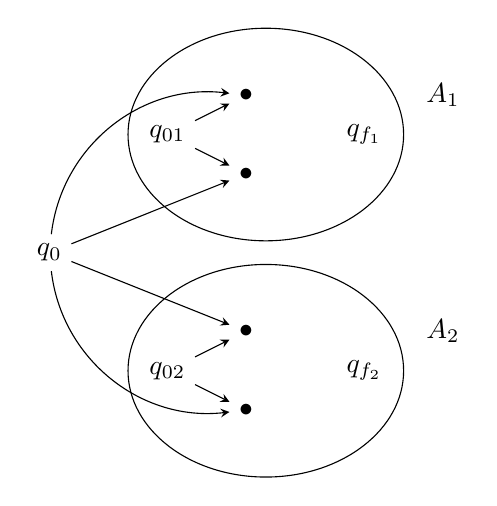
\begin{tikzpicture}[>=stealth]
                \node (q0) at (0,0) {$q_0$};
                
                \node (q01) at (1.5,1.5) {$q_{01}$};
                \node (y) at (2.5,2) {$\bullet$};
                \node (x1) at (2.5,1) {$\bullet$};
                \node (qf1) at (4,1.5) {$q_{f_1}$};
                
                \node (q02) at (1.5,-1.5) {$q_{02}$};
                \node (x2) at (2.5,-1) {$\bullet$};
                \node (l) at (2.5,-2) {$\bullet$};
                \node (qf2) at (4,-1.5) {$q_{f_2}$};
                
                \path [->] (q0) edge [bend left=45] (y)
                                edge (x1)
                                edge (x2)
                                edge [bend right=45] (l)
                          (q01) edge (y)
                                edge (x1)
                          (q02) edge (x2)
                                edge (l)
%                ;
%                \path (q01) edge [bend left=80] (qf1)
%                                    edge [bend right=80] (qf1)
                ;\draw (2.75,-1.5) ellipse (1.75 and 1.35);
                \node at (5,2) {$A_1$}
                ;
                \draw (2.75,1.5) ellipse (1.75 and 1.35);
                \node at (5,-1) {$A_2$};
            \end{tikzpicture}
            \caption{\acs{NFA} f"ur Vereinigung}
            \label{fig:reg-closure-union}
        \end{figure}
		DFA:
		\begin{align*}
			Q &= Q_1\x Q_2\\
			\delta((q_1,q_2),a) &= (\delta_1(q_1,a),\delta_2(q_2,a))\\
			q_0 &= (q_{01},q_{02})\\
			F &= F_1\x F_2\\
			\text{Zeige }L(\A) &= &L(\A_1)\cap L(\A_2)
		\end{align*}
	\item Komplement: Ang. $\A_1$ ist \ac{DFA}.\\
		Ersetze $F_1$ durch $Q_1\setminus F_1$.
%
%
	\item Produkt: Seien $L_1$, $L_2$ regulär.\\
		Zeige $L_1\cdot L_2$ regulär.
		\begin{align*}
			Q &= Q_1 \overset.\cup Q_2\\
			\delta(q,a) &=
				\begin{cases}
					\delta_1(q,a) & q\in Q_1\setminus F_1\\
					\delta_1(q,a)\cup\delta_2(q_{02},a) & q\in F_1\\
					\delta_2(q,a) & q\in Q_2
				\end{cases}\\
		q_0& = q_{01}\\
		F &= F_2\cup(q_{02}\in F_2) \rhd F_1
		\end{align*}
		Zeige $L(\A) = L(\A_1)\cdot L(A_2)$
	\item Stern
	\begin{align*}
		Q &= Q_1\overset.\cup \{q_0\}\\
		\delta(q,a) &=
			\begin{cases}
				\delta_1(q,a) & q\in Q_1\setminus F_1\\
				\delta_1(q,a)\cup\delta_1(q_{01},a) & q\in F_1\\
				\delta_1(q_{01},a) & q=q_0
			\end{cases}\\
		F &= \{q_0\}\cup F_1\\
		\dots\ L(\A) &= L(\A_1)^*
	\end{align*}
	\end{itemize}
\end{proof}
%
\subsection{Reguläre Ausdrücke}
\draftnote{4.11.16}
\begin{Def}[name={[RE($\Sigma$)]}]
	Die Menge $RE(\Sigma)$ der \emph{regulären Ausdrücke über $\Sigma$} ist induktiv definiert durch:
	\begin{itemize}
	\item $\0\in RE(\Sigma)$
	\item $\1\in RE(\Sigma)$
	\item $\forall a\in\Sigma$, $a\in RE(\Sigma)$
	\item falls $r,s\in RE(\Sigma)$
		\begin{itemize}[label=\textbullet]
		\item $r+s\in RE(\Sigma)$
		\item $r\cdot s\in RE(\Sigma)$
		\item $r^*\in RE(\Sigma)$
		\end{itemize}
	\end{itemize}
\end{Def}
\begin{Def}[name={[Semantik eines regulären Ausdrucks]}]
	Die Semantik eines regulären Ausdrucks
	\begin{align*}
		\llbracket\cdot \rrbracket &: RE(\Sigma) \-> \mathcal{P}(\Sigma^*)\text{ ist induktiv def. durch}\\
		\llbracket \0 \rrbracket &= \varnothing\\
		\llbracket \1 \rrbracket &= \{\Eps\}\\
		\llbracket a \rrbracket &= \{a\} \quad a\in\Sigma\\
		\llbracket r+s \rrbracket &= \llbracket r\rrbracket \cup \llbracket s\rrbracket\\
		\llbracket r\cdot s \rrbracket &= \llbracket r\rrbracket \cdot \llbracket s\rrbracket\\
		\llbracket r^* \rrbracket &= \llbracket r\rrbracket^* \qedhere
	\end{align*}
\end{Def}
$+,\cdot ,*$ reguläre Operatoren.\\
%
\begin{minipage}[t]{.5\textwidth}
    \begin{Bsp*} Mustererkennung
    	\begin{itemize}
    	\item $\underset{\vphantom{\big(}\mathrlap{\hspace{-4pt}\rotatebox[origin=c]{90}{$\Rsh$}\ =(a_1+a_2+\dots) \text{ alle $a_i\in\Sigma$ aufgez"ahlt}}}{\Sigma^*}\ abac\ \Sigma^*$
    	\item $n$-letztes Symbol = 1 ($\Sigma=\{0,1\}$)
    	\begin{gather*}
    	(0+1)^*1\underbrace{(0+1)\dots(0+1)}_{n-1}\\
    	\xcancel{0^n1^n}\notin RE(\Sigma)
    	\end{gather*}
    	\item Binärdarstellung modulo $3=0$
    	\[ (0+1(01^*0)^*1)^* \]
    	\end{itemize}
    \end{Bsp*}
\end{minipage}%
\begin{minipage}[t]{.5\textwidth}
    \vspace{0pt}
    \captionsetup{type=figure}
    \begin{tikzpicture}[>=stealth, shorten >=1pt, on grid, node distance=2cm, initial text=]
        \node[state, initial, accepting] (q0) {$q_0$};
        \node[state] (q1) [right=of q0] {$q_1$};
        \node[state] (q2) [right=of q1] {$q_2$};
        \path [->]
            (q0) edge[loop below] node[auto] {0} ()
                 edge[bend left]  node[auto] {1} (q1)
            (q1) edge[bend left]  node[auto] {0} (q2)
                 edge[bend left]  node[auto] {1} (q0)
            (q2) edge[loop right] node[auto] {1} ()
                 edge[bend left]  node[auto] {0} (q1)
        ;
        
        \draw [->,decorate,decoration=snake] ($(q1.south) - (0,.5cm)$) -- ++(0,-1cm);
        
        \node [state, initial, accepting] (q0) [below=3cm of q0] {$q_0$};
        \node [state] (q1) [right=of q0] {$q_1$};
        \path [->]
            (q0) edge[loop below] node[auto] {0} ()
                 edge[bend left]  node[auto] {1} (q1)
            (q1) edge[loop right] node[auto] {$01^*0$} ()
                 edge[bend left]  node[auto] {1} (q0)
        ;
        
        \node [state, initial, accepting] (q0) [below=2.5cm of q0] {$q_0$};
        \path [->]
            (q0) edge[loop below] node[auto] {0} ()
                 edge[loop right] node[auto] {$1(01^*0)^*1$} ()
        ;
    \end{tikzpicture}
    \captionof{figure}{Informell vom Automaten zum regul"aren Ausdruck f"ur mod 3}
\end{minipage}

\begin{Satz}[Kleene]
$L$ ist regulär\\
\<=> $L$ ist Sprache eines regulären Ausdrucks.
\end{Satz}
\begin{proof}\
	\begin{description}[labelwidth=\widthof{\<=},leftmargin=!]
	\item["`\<="'] Sei $L=\llbracket r \rrbracket$ für $r\in RE(\Sigma)$\\
		Zeige per Induktion über $r: \forall r\in RE(\Sigma) : \llbracket r \rrbracket$ regulär.
    	\begin{description}[font=\normalfont]
    		\setlength{\abovedisplayskip}{-1em}
    		\item[I.A.:]
    		\begin{align*}
    			\0 &: \varnothing\text{ ist reg.}\\
    			\1 &: \{\Eps\}\text{ ist reg.}\\
    			a &: \{a\} \tikz[>=stealth, shorten >=1pt, initial text=,
    					on grid, baseline=-.6ex,
    					every state/.style={minimum size=0pt,inner sep=0pt}
    				]{
    				\node [state,initial] (a) {}; \node [state,accepting] (b) [right=of a] {};
    				\path [->] (a) edge node [auto] {a} (b);
    			}
    			 \quad\acs{NFA}
    		\end{align*}
    		\item[I.S.:]
    		{\settowidth{\dimen1}{reg. nach \autoref{satz:3.8}}
    		\begin{alignat*}{3}
    			r+s &:{}& \llbracket r+s \rrbracket &= \llbracket r \rrbracket \cup \llbracket s \rrbracket &\quad &\text{reg. nach \autoref{satz:3.8}}\\
    			r\cdot s &:& \llbracket r\cdot s \rrbracket &= \llbracket r \rrbracket\cdot \llbracket s \rrbracket && \ruleplaceholder{\dimen1}\\
    			r^* &:& \llbracket r* \rrbracket &= \llbracket r \rrbracket^* && \ruleplaceholder{\dimen1}
    		\end{alignat*}}
		\end{description}
	\item["`\=>"'] Sei $L=L(\A)$ für einen \ac{DFA} $\A=(\underoverbrace{=\{q_0,q_1,\dots,q_n\}}{Q},\Sigma,\delta,q_0,F)$.\\[.5em]
		Def. $L_i=\{ w \mid \hat\delta(q_i,w)\in F \}$\quad(Also $L(\A)=L_0$)
		\begin{alignat*}{2}
			&\text{Betrachte }\quad & \delta(q_i,a) &=q_j\\
			&\quad\curvearrowright & L_i &\supseteq a_i\cdot L_j\\
			&\text{Betrachte} &  & \text{alle Transitionen ab }q_i \\
			&\quad\curvearrowright & L_i &= N(q_i)+\sum_{0 \le j \le n} A_{ij}\cdot L_j\\
			&& A_{ij} &= \sum_{a \in \Sigma, \delta(q_i,a) = q_j} a \\
			&& N(q_i) &= 
				\begin{cases}
					\1 &, q_i\in F\\
					\0 &, q_i\notin F
				\end{cases}
		\end{alignat*}
		Also: $\A$ berechnet die Lösung eines Gleichungssystems
		\[ L_i=N(q_i) + \sum_j A_{ij}L_j \quad\text{mit }\Eps\notin A_{ij} \]
		Zur L"osung dieses Gleichungssystems verwenden wir das Lemma von Arden:
	\end{description}
\end{proof}
\begin{lemma}[Arden's Lemma]\label{lem:arden}\ \\
	Sei $X=A\cdot X+B$ für $\underset{\vphantom{\big(}\ \mathrlap{\hspace{-4pt}\rotatebox[origin=c]{90}{$\Rsh$}\ \text{Unbekannte}}}{X} ,A,B\subseteq \Sigma^*$\\
	dann ist $X=A^*B$ falls $\Eps\notin A$.
%	\begin{align*}
%		&& B &\subseteq X\\
%		&& B+AB &\subseteq X\\
%		X&=\Eps\cdot X+B & AAB &\subseteq X\\
%		&& \forall n : A^nB &\subseteq X
%	\end{align*}
\end{lemma}
\begin{proof}[Fortsetzung]
    Verfahren zur L"osung des Gleichungssystems:
    
	Eliminiere sukzessive die Gleichung für $L_n$ (bis nur noch eine Gleichung f"ur $L_0$ "ubrig ist)
	\begin{enumerate}[label=(\arabic*)]
		\item Falls Gleichung für $L_n$ rekursiv
			\begin{align*}
				\text{dann hat sie die Form}:\quad L_n &= \underbrace{\Big( N(q_n)+\sum_{j\neq n} A_{nj}\cdot L_j \Big)}_{=: B} + \underbrace{A_{nn}}_{=: A \not\ni \Eps}\cdot L_n\\
				\text{Nach Ardens Lemma}:\quad L_n &= A_{nn}^*\cdot \Big( N(q_n)+\sum_{j\neq n} \underbrace{A_{nj}}_{\not\ni\Eps} \cdot L_j \Big)\\
				&= A_{nn}^*\cdot N(q_n) + \sum_{j\neq n} \underbrace{A_{nn}^*\cdot A_{nj}}_{\not\ni\Eps} \cdot L_j
			\end{align*}
			Gleichungssystem der gleichen Form: linear in den $L_j$ mit Koeffizienten, die nicht $\Eps$ enthalten.
		\item Gleichung für $L_n$ nicht rekursiv:\\
		Setze rechte Seite für $L_n$ in die Gleichungen $L_0, L_1, \dots, L_{n-1}$ ein. \--> Gleichungssystem der gleichen Form.
	\end{enumerate}
    Nach $n+1$ Iterationen erhalten wir ein Gleichungssytem der Form $L_0=r$. \hfill$\bigoplus$
\end{proof}
\begin{proof}(Arden's Lemma)
	\begin{alignat*}{3}
		\text{Sei}&\quad& X&= AX+B\text{ mit }\Eps\notin A.\\
		\text{Zeige}&& A^*B&\subseteq X.\\
		&& A^*B &= (\1+AA^*)B = B+A(A^*B) \quad\checkmark\\
		\shortintertext{Angenommen $A^*B \subsetneq X$, d.h. $\exists w\in X$ mit $w\notin A^*B$, davon sei $w$ das kürzeste.}
		\exists n\geq 1: && X &= \underbrace{A^nX}_{\ni w} + \underbrace{A^{n-1}B+\dots +AB+B}_{\not\ni w}\\
		\curvearrowright && w &= u_1\dots u_n w'\text{ mit } u_1,\dots,u_n\in A\text{ und } w'\in X\\
		\curvearrowright && |w'| &< |w|\\
		\text{Falls}&& w'&\in A^*B \curvearrowright w\in A^nA^*B\subseteq A^*B \quad \lightning\\
		\text{Also} && w'&\notin A^*B \quad\lightning\text{ gegen Minimalität von }w\\
		\curvearrowright && X&\subseteq A^*B\\
		\-> && X &= A^*B \tag*{\qedhere}
	\end{alignat*}
\end{proof}

\begin{Bsp*} für Konv. \ac{DFA}\-> $RE$
	\begin{figure}[H]\centering
		\begin{tikzpicture}[>=stealth, shorten >=1pt, on grid, node distance=2cm, initial text=]
			\node[state, initial, accepting] (q0) {$q_0$};
			\node[state] (q1) [right=of q0] {$q_1$};
			\node[state] (q2) [right=of q1] {$q_2$};
			\path [->]
			    (q0) edge[loop above] node[auto] {0} ()
			         edge[bend left]  node[auto] {1} (q1)
			    (q1) edge[bend left]  node[auto] {0} (q2)
			         edge[bend left]  node[auto] {1} (q0)
			    (q2) edge[loop right] node[auto] {1} ()
			         edge[bend left]  node[auto] {0} (q1)
			;
		\end{tikzpicture}
		\caption{\ac{DFA} "`modulo 3"'}
	\end{figure}
	lineares Gleichungssystem mit 3 Unbekannten.
	\begin{align*}
		L_0 &= \1 + 0\cdot L_0 + 1\cdot L_1\\
		L_1 &= 1\cdot L_0 + 0\cdot L_2\\
		L_2 &= \underbrace{0\cdot L_1}_B + \underbrace{1}_A\cdot L_2\\
		\shortintertext{\nameref{lem:arden} auf $q_2$:}
		L_2 &= 1^*\cdot 0\cdot L_1\\
		\shortintertext{Einsetzen in $q_1$}
		L_1 &= \underbrace{1\cdot L_0}_B+\underbrace{0\cdot 1^*\cdot 0}_A\cdot L_1\\
		\shortintertext{\nameref{lem:arden} auf $q_1$:}
		L_1 &= (01^*0)^*\cdot 1\cdot L_0\\
		\shortintertext{Einsetzen:}
		L_0 &= \1 + 0\cdot L_0+1\cdot (01^*0)^*\cdot 1\cdot L_0\\
		&= \1+(0+1\cdot (01^*0)^*\cdot 1)\cdot L_0\\
		\shortintertext{\nameref{lem:arden} auf $q_0$:}
		L_0 &= (0+1\cdot (01^*0)^*\cdot 1)^*
	\end{align*}
\end{Bsp*}
%
\subsection{Entscheidungsprobleme}
\begin{Satz}[name={[Wortproblem]}]\label{satz:wortproblem}
	Das Wortproblem ist für reguläre Sprachen entscheidbar.
	
	D.h. Falls $L$ reg. Sprache und $w\in\Sigma^*$, dann ex. Algorithmus, der entscheidet, ob $w\in L$.
\end{Satz}
\begin{proof}
	$L$ sei durch \ac{DFA} gegeben.\\
	Berechnung von $\hat\delta(q_0,w)$ entspricht Durchlauf durch Graph des \ac{DFA} + Test ob erreichter Zustand $\in F$ in Zeit $O(n)\ ,\ n=|w|$.
\end{proof}

\begin{Satz}[name={[Leerheitsproblem]}]\label{satz:leerheitsproblem}
	Das \emph{Leerheitsproblem} ist für reg. Sprachen entscheidbar.
	Falls $L$ reg. Sprache, dann existiert ein Algorithmus, der entscheidet, ob $L=\varnothing$.
\end{Satz}
\begin{proof}
	Sei $\A$ \ac{DFA} für $L$.\\
	Setze Tiefensuche auf den Graphen von $\A$ an. Start bei $q_0$.\\
	Falls die Suche einem akzeptierenden Zustand findet: Nein.\\
	Ansonsten: Ja: $L=\varnothing$\\
	Zeit: $O(|\Sigma||Q|)$
	\rlwarning{Beweis vollständig?}
\end{proof}

\begin{Satz}[name={[Endlichkeitsproblem]}]\label{satz:endlichkeitsproblem}
	Das Endlichkeitsproblem für reg. Sprachen ist entscheidbar.
\end{Satz}
\begin{proof}
	Falls $L$ durch $r\in RE(\Sigma)$ gegeben.\\
	$r$ enthält keinen $^* \=> \llbracket r \rrbracket$ endlich.\\
	Zeit: $O(|r|)$
	
	[Reicht nicht, liefert nur eine Richtung]
	
	Falls $L$ durch \ac{DFA} $\A$ gegeben.
	
	\begin{tikzpicture}[>=stealth]
		\node (q0) {$q_0$};
		\node (q1)  [right=.75cm of q0]{$\cdot$};
		\node (q2) [right=.48cm of q1] {$\times$};
		\node (q3) [below=.4cm of q2, xshift=.4cm, inner sep=0pt] {$\times$};
		\draw[->] (q0) edge (q1)
			(q2) ++(-.1cm,-.3cm) -- (q3);
		\draw[->] (q1.south) arc (-155:155:.5cm);
	\end{tikzpicture}
	
	\paragraph*{Oder:} mit \nameref{lem:pumping}.\\
	Sei $L$ regulär und $n$ die Konstante aus dem \ac{PL}.\\
	$L$ unendlich \<=> $\exists w\in L : n\leq |w| <2n$
	\begin{description}[font=\normalfont,labelwidth=\widthof{"'\<="':},leftmargin=!]
	\item["'\<="':] $w$ erfüllt Voraussetzung des \ac{PL}, also $w=uvx$ mit $|uv|\leq n$ und $|v|\geq 1$.\\
		Nach \ac{PL}: $\forall i\in\N$, $uv^ix\in L$, also $L$ unendlich.
	\item["'\=>"'] \emph{Angenommen} $L$ unendlich, aber $\forall w\in L : |w|<n$ oder $|w|\geq 2 n$\\
	Sei $w\in L$ minimal gewählt, so dass $|w|\geq 2n$.
	
	$w$ erfüllt Voraussetzung vom \ac{PL}, also $w=xyz$ mit $|xy|\leq n$ und $|y|\geq 1$\\
	also $\forall i\in\N: xy^iz\in L$ insbes. $i=0: xz\in L$ mit $|xz|<|w|$.
	
	Zwei Möglichkeiten:
	\begin{enumerate}[label=(\alph*)]
	\item $|xz|\geq 2n\ \lightning$ Minimalität von $w$
	\item $|xz|<2n$
		\begin{align*}
			|xz|+|y| &= |w|\geq 2n\text{ mit } 1\leq|y|\leq n\\
			\curvearrowright |xz| &= |w|-|y|\geq 2n-n=n \quad\lightning\text{ zur Annahme}
		\end{align*}
		Also $\exists w\in L$ mit $n\leq|w|<2n$ \qedhere
	\end{enumerate}
	\end{description}
\end{proof}

\begin{Satz}[name={[Schnittproblem]}]\label{satz:schnittproblem}
	Das \emph{Schnittproblem} ist für REG entscheidbar.\\
	D.h. $L_1,L_2$ reguläre Sprachen. Ist $L_1\cap L_2 = \varnothing$?
\end{Satz}
\begin{proof}
	Nach Satz \ref{satz:schnittproblem} ist $L_1\cap L_2$ regulär. $L_1\cap L_2=\varnothing$ entscheidbar nach \autoref{satz:leerheitsproblem}.
\end{proof}

\begin{Satz}[name={[Äquivalenzproblem]}]\label{satz:äquivalenzproblem}
	Das \emph{Äquivalenzproblem} ist für REG entscheidbar.\\
	D.h. gegeben \ac{DFA}s für $L_1$ und $L_2$, $\A_1$ und $\A_2$
	\[ L_1 = L(\A_1) = L(\A_2) = L_2\ ? \qquad \framebox{Inklusionsproblem}\]
\end{Satz}
\vspace{-2em}
\begin{proof}
	\begin{alignat*}{3}
		L_1\cap \overline{L}_2 &= \varnothing &\quad&\<=>\quad & L_1 &\subseteq L_2\\
		(L_1\cap\overline{L}_2)\cup(L_2\cap \overline{L}_1) &= \varnothing &&\<=> & L_1 &= L_2 \tag*{\qedhere}
	\end{alignat*}
\end{proof}

\begin{Satz}[name={[Inklusionsproblem]}] Äquivalenzproblem \<=> Inklusionsproblem (für REG)
\end{Satz}
\begin{proof}
\begin{itemize}
\item  $=$ entspricht $\subseteq\land\supseteq$
\item $L_1 \subseteq L_2$ genau dann, wenn $L_1 \cup L_2 = L_2$; REG ist abgeschlossen unter Vereinigung
\end{itemize}
\end{proof}


Anwendungsbeispiel f"ur regul"are Sprachen.

$N$ -- liest vom Netz\\
$R$ -- liest lokalen Speicher (ggf. vertrauliche Info)\\
$W$ -- postet auf FB

Programm:

\begin{tabular}{M{l}@{}M{l}@{}M{l}}
	p = N | R | W &| \text{ if }&* \text{ then } p_1\\
	&&\phantom{*}\text{ else }p_2\\
	&|\text{ while }&*\text{ do }p\\
	\mathrlap{
		\begin{rcases}
			\text{while }*\text{ do }N;\\
			R;\\
			\text{if }*\text{ then }N\text{ else }W
		\end{rcases} N^*R\cdot (N+W)
	}
\end{tabular}

Sicherheitspolitik: nach Lesen von lokalem Speicher kein Posten auf FB  $\overline{\Sigma^*R\Sigma^*W\Sigma^*}$

Programm erfüllt Sicherheitspolitik nicht, denn
\[
	\underset{\underset{\displaystyle N^*RW}{\rotatebox[origin=c]{-90}{$\supseteq$}}}{N^*\cdot R(N+W)} \not\subseteq \overline{\Sigma^*R\Sigma^*W\Sigma^*}
\]